% Graphical Abstract - Healthcare Analytics
% Compile with pdflatex; export to TIFF/EPS/PDF/PNG for submission.
\documentclass[12pt]{article}
\usepackage[margin=0.05in,paperwidth=20cm,paperheight=9.5cm]{geometry}
\usepackage{tikz}
\renewcommand{\familydefault}{\sfdefault}
\usetikzlibrary{arrows.meta,positioning,shapes.geometric}
\pagestyle{empty}

\tikzset{
  pics/person/.style={code={
    \fill[blue!60] (0,0.62) circle (0.30);
    \fill[blue!45] (-0.55,0.05) .. controls (-0.55,-0.60) and (0.55,-0.60) .. (0.55,0.05) -- (-0.55,0.05) -- cycle;
  }},
  pics/doc/.style={code={
    \draw[fill=white, draw=blue!55, rounded corners=2pt, line width=0.8pt] (-0.38,-0.52) rectangle (0.38,0.52);
    \draw[blue!45] (-0.20,0.24) -- (0.20,0.24);
    \draw[blue!45] (-0.20,0.04) -- (0.20,0.04);
    \draw[blue!45] (-0.20,-0.16) -- (0.20,-0.16);
  }},
  pics/checkdoc/.style={code={
    \draw[fill=white, draw=green!50!black, rounded corners=2pt, line width=1pt] (-0.4,-0.6) rectangle (0.3,0.5);
    \node[font=\small\bfseries, text=green!50!black, anchor=west] at (-0.35, 0.25) {A};
    \draw[green!50!black, line width=1pt] (-0.3,-0.05) -- (0.2,-0.05);
    \draw[green!50!black, line width=1pt] (-0.3,-0.25) -- (0.2,-0.25);
    \draw[green!50!black, line width=1pt] (-0.3,-0.45) -- (-0.05,-0.45);
    \fill[green!50!black] (0.3,-0.4) circle (0.22);
    \draw[white, line width=1.5pt] (0.18,-0.4) -- (0.26,-0.5) -- (0.42,-0.3);
  }},
  pics/manifold/.style={code={
    \draw[teal!70!black, thick] (-0.95,0) .. controls (-0.45,0.95) and (0.45,0.95) .. (0.95,0)
      .. controls (0.45,-0.95) and (-0.45,-0.95) .. (-0.95,0);
    \fill[teal!70!black] (-0.55,0.47) circle (1.8pt);
    \fill[teal!70!black] (0.0,0.72) circle (1.8pt);
    \fill[teal!70!black] (0.55,0.47) circle (1.8pt);
    \draw[->, teal!70!black, line width=1pt] (0.0,0.72) -- (0.42,0.82);
  }},
  pics/gate/.style={code={
    \draw[orange!80!black, line width=1pt] (-0.42,-0.55) -- (-0.42,0.55);
    \draw[orange!80!black, line width=1pt] (0.42,-0.55) -- (0.42,0.55);
    \draw[orange!80!black, line width=1pt] (-0.42,0.55) -- (0.42,0.55);
    \draw[rotate around={18:(0.42,-0.55)}, fill=orange!35, draw=orange!80!black, line width=0.8pt]
      (0.42,-0.55) rectangle (0.62,0.55);
    \fill[orange!90!black] (0,0) circle (1.5pt);
  }},
  pics/jepa/.style={code={
    \draw[green!70!black, line width=1.2pt] (0,0) circle (0.46);
    \draw[green!70!black, line width=1pt] (0,0) -- (0,0.16) -- (0.14,0.28);
    \draw[->, green!70!black, line width=1.2pt] (0.45,0.35) -- (0.95,0.35);
    \draw[green!70!black, line width=1pt] (0.62,0.55) -- (0.74,0.55);
  }},
  pics/speed/.style={code={
    \draw[purple!70!black, line width=3.5pt] (0.6,0) arc (0:180:0.6);
    \draw[purple!70!black, line width=3pt, rounded corners=1pt] (-0.05,-0.1) -- (0.35,0.45);
  }},
  pics/medal/.style={code={
    \draw[green!50!black, line width=1.2pt] (-0.18,-0.2) -- (-0.35,-0.65) -- (-0.15,-0.55) -- (-0.05,-0.65) -- (0,-0.3);
    \draw[green!50!black, line width=1.2pt] (0.18,-0.2) -- (0.35,-0.65) -- (0.15,-0.55) -- (0.05,-0.65) -- (0,-0.3);
    \draw[fill=white, draw=green!50!black, line width=1.2pt] (0,0) circle (0.35);
    \draw[draw=green!50!black, line width=0.8pt] (0,0) circle (0.28);
    \node[font=\tiny\bfseries, text=green!50!black] at (0,0) {100\%};
  }},
  panel/.style={rounded corners=8pt, draw, line width=1.1pt},
  hdr/.style={font=\small\bfseries, text=black!85, text width=5.2cm, align=center},
  lab/.style={font=\small, text=black!85},
  sublab/.style={font=\scriptsize, text=black!70, align=center},
  subtitle/.style={font=\scriptsize, text=black!60, text width=5.2cm, align=center},
  arr/.style={-{Stealth[length=4.5mm]}, line width=1.4pt, color=black!60}
}

\begin{document}
\noindent
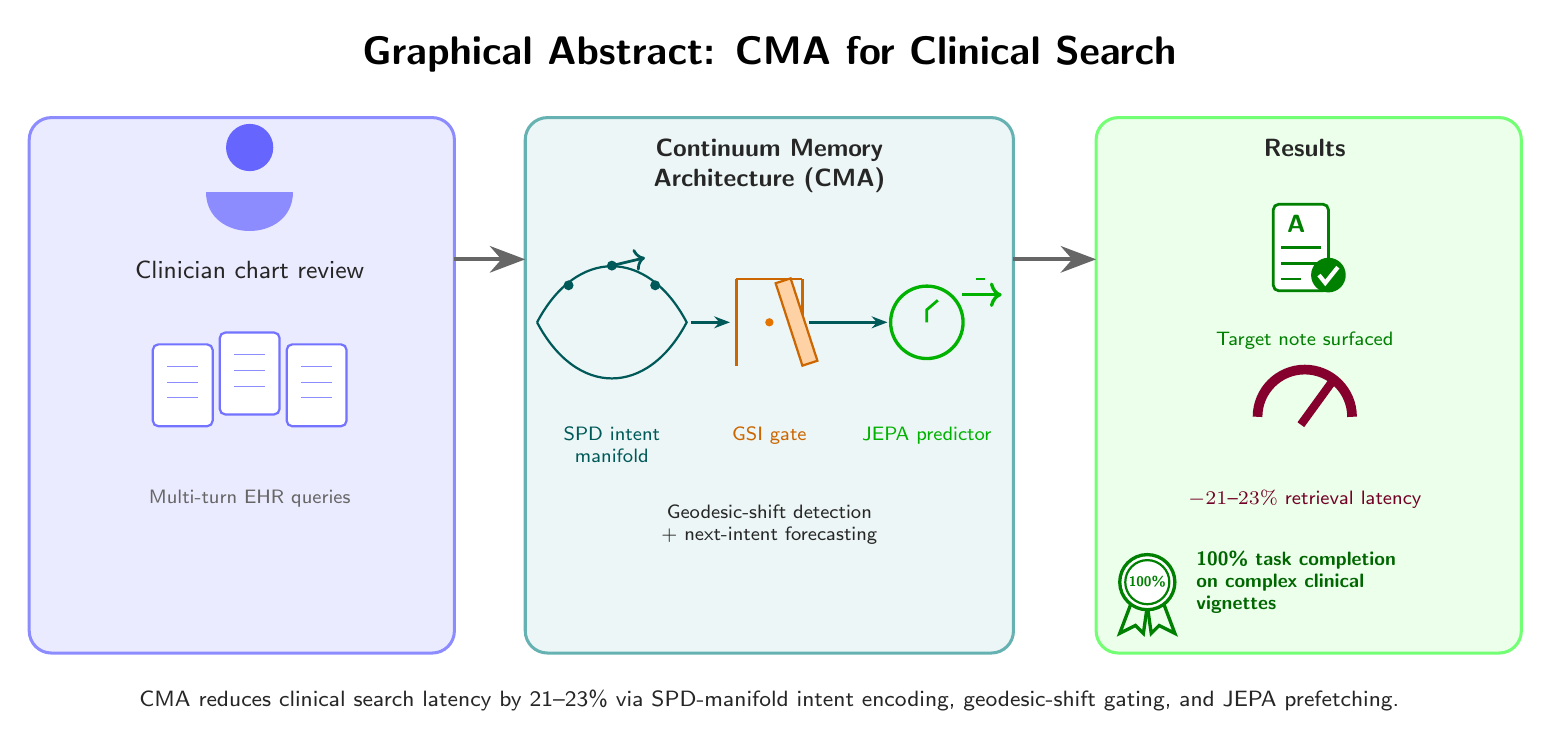
\begin{tikzpicture}[x=1cm,y=1cm]

% ---------------- Title ----------------
\node[font=\Large\bfseries, text=black] at (10.2, 8.8) {Graphical Abstract: CMA for Clinical Search};

% ---------------- Panel 1: clinician chart review ----------------
\node[panel, fill=blue!8, draw=blue!45, minimum width=5.4cm, minimum height=6.8cm] (p1) at (3.5,4.6) {};
\draw (3.6,7.0) pic {person};
\node[lab, anchor=north] at (3.6,6.3) {Clinician chart review};
\draw (2.75,4.6) pic {doc};
\draw (3.6,4.75) pic {doc};
\draw (4.45,4.6) pic {doc};
\node[subtitle, anchor=north] at (3.6,3.4) {Multi-turn EHR queries};

% ---------------- Panel 2: CMA ----------------
\node[panel, fill=teal!7, draw=teal!60, minimum width=6.2cm, minimum height=6.8cm] (p2) at (10.2,4.6) {};
\node[hdr, anchor=north] at (10.2,7.85) {Continuum Memory\\Architecture (CMA)};

\draw (8.2,5.4) pic {manifold};
\node[sublab, anchor=north, text=teal!70!black, text width=2.2cm] at (8.2,4.2) {SPD intent\\manifold};
\draw (10.2,5.4) pic {gate};
\node[sublab, anchor=north, text=orange!80!black] at (10.2,4.2) {GSI gate};
\draw (12.2,5.4) pic {jepa};
\node[sublab, anchor=north, text=green!70!black, text width=2.1cm] at (12.2,4.2) {JEPA predictor};

\draw[-{Stealth[length=2mm]}, teal!70!black, line width=1pt] (9.2,5.4) -- (9.7,5.4);
\draw[-{Stealth[length=2mm]}, teal!70!black, line width=1pt] (10.7,5.4) -- (11.7,5.4);

\node[subtitle, anchor=north, text=black!85] at (10.2,3.2) {Geodesic-shift detection\\+ next-intent forecasting};

% ---------------- Panel 3: results ----------------
\node[panel, fill=green!8, draw=green!55, minimum width=5.4cm, minimum height=6.8cm] (p3) at (17.05,4.6) {};
\node[hdr, anchor=north] at (17.0,7.85) {Results};

\draw (17.0,6.4) pic {checkdoc};
\node[sublab, anchor=north, text=green!50!black] at (17.0,5.4) {Target note surfaced};

\draw (17.0,4.2) pic {speed};
\node[sublab, anchor=north, text=purple!60!black] at (17.0,3.4) {$-21$--$23\%$ retrieval latency};

\draw (15.0,2.1) pic {medal};
\node[sublab, anchor=west, font=\scriptsize\bfseries, text=green!40!black, text width=3.4cm, align=left] at (15.5,2.1) {100\% task completion\\on complex clinical\\vignettes};

% ---------------- Inter-panel arrows ----------------
\draw[arr] (6.2,6.2) -- (7.1,6.2);
\draw[arr] (13.3,6.2) -- (14.35,6.2);

% ---------------- Caption ----------------
\node[font=\footnotesize, text=black!85, text width=18cm, align=center] at (10.2,0.6)
  {CMA reduces clinical search latency by 21--23\% via SPD-manifold intent encoding, geodesic-shift gating, and JEPA prefetching.};

\end{tikzpicture}
\end{document}